\documentclass[10pt]{extarticle}
\usepackage{main}
\usepackage{libertinus}
\usepackage[T1]{fontenc}
\usepackage{multicol}
\usepackage{graphicx}
\graphicspath{ {images/} }

\begin{document}
\begin{exercise}
    \dots the weights may be reduced to zero.
    \begin{choice}(4)
        * L1 and L2
        * \correctchoice{L1}
        * L2
        * None of the above
    \end{choice}
\end{exercise}
\begin{solution}
\end{solution}

\begin{exercise}
    Bagging is an ensemble technique that:
    \begin{choice}
        * Combines predictions using a weighted average
        * \correctchoice{Trains multiple models on different subsets of the data}
        * Constructs an ensemble by iteratively updating weights
        * Uses a committee of experts to make predictions
    \end{choice}
\end{exercise}
\begin{solution}
\end{solution}

\begin{exercise}
    Which of the following is/are Limitations of deep learning?
    \begin{choice} (2)
        * Data labeling
        * Obtain huge training datasets
        * \correctchoice{Both \circled{A} and \circled{B}}
        * None of the previous
    \end{choice}
\end{exercise}
\begin{solution}
\end{solution}

\begin{exercise}
    Which neural network has only one hidden layer between the input and output?
    \begin{choice} (2)
        * \correctchoice{Shallow neural network}
        * Deep neural network
        * Feed-forward neural networks
        * Recurrent neural networks
    \end{choice}
\end{exercise}
\begin{solution}
\end{solution}

\begin{exercise}
    CNN is mostly used when there is an?
    \begin{choice} (4)
        * structured data
        * \correctchoice{unstructured data}
        * both \circled{A} and \circled{B}
        * None of the previous
    \end{choice}
\end{exercise}
\begin{solution}
\end{solution}

\begin{exercise}
    Which of the following is well suited for perceptual tasks?
    \begin{choice} (1)
        * feed-forward neural networks
        * recurrent neural networks
        * \correctchoice{convolutional neural networks}
        * Reinforcement learning
    \end{choice}
\end{exercise}
\begin{solution}
\end{solution}

\begin{exercise}
    Which of the following is/are Common uses of RNNs?
    \begin{choice}
        * BusinessesHelp securities traders to generate analytic reports
        * Detect fraudulent credit-card transaction
        * Provide a caption for images
        * \correctchoice{All of the above}
    \end{choice}
\end{exercise}
\begin{solution}
\end{solution}

\begin{exercise}
    Boosting is an ensemble technique that:
    \begin{choice}
        * Combines predictions using a weighted average
        * Trains multiple models on different subsets of the data
        * \correctchoice{Constructs an ensemble by iteratively updating weights}
        * Uses a committee of experts to make predictions
    \end{choice}
\end{exercise}
\begin{solution}
\end{solution}

\begin{exercise}
    What steps can we take to prevent overfitting in a Neural Network?
    \begin{choice}(2)
        * Data Augmentation
        * Weight Sharing
        * Early Stopping
        * Dropout
        * \correctchoice{All of the previous}
    \end{choice}
\end{exercise}
\begin{solution}
\end{solution}

\begin{exercise}
    Which of the following is an example of an ensemble learning algorithm?
    \begin{choice} (4)
        * Decision tree
        * SVM
        * \correctchoice{Random Forest}
        * KNN
    \end{choice}
\end{exercise}
\begin{solution}
\end{solution}

\begin{exercise}
    AdaBoost is an example of:
    \begin{choice} (2)
        * Bagging algorithm
        * \correctchoice{Boosting algorithm}
        * Randomized algorithm
        * Reinforcement learning algorithm
    \end{choice}
\end{exercise}
\begin{solution}
\end{solution}

\begin{exercise}
    Gradient Boosting is an ensemble technique that:
    \begin{choice}
        * Combines predictions using a weighted average
        * Trains multiple models on different subsets of the data
        * \correctchoice{Constructs an ensemble by iteratively updating weights}
        * Uses a committee of experts to make predictions
    \end{choice}
\end{exercise}
\begin{solution}
\end{solution}

\begin{exercise}
    XGBoost is a popular implementation of:
    \begin{choice}(2)
        * Bagging algorithm
        * \correctchoice{Boosting algorithm}
        * Random Forest Algorithm
        * K-Means clustering algorithms
    \end{choice}
\end{exercise}
\begin{solution}
\end{solution}

\begin{exercise}
    Stacking is an ensemble technique that:
    \begin{choice} (1)
        * Combines predictions using a weighted average
        * Trains multiple models on different subsets of the data
        * Constructs an ensemble by iteratively updating weights
        * \correctchoice{Trains a meta-model to make predictions based on outputs of base models}
    \end{choice}
\end{exercise}
\begin{solution}
\end{solution}

\begin{exercise}
    Which ensemble learning algorithm uses bootstrapping and feature sampling?
    \begin{choice} (4)
        * \correctchoice{Random Forest}
        * AdaBoost
        * Gradient Boosting
        * Stacking
    \end{choice}
\end{exercise}
\begin{solution}
\end{solution}

\begin{exercise}
    The purpose of using ensemble learning is to:
    \begin{choice}
        * \correctchoice{Reduce overfitting and improve generalization}
        * Increase training time and complexity
        * Decrease the number of models required
        * Eliminate the need for labeled data
    \end{choice}
\end{exercise}
\begin{solution}
\end{solution}

\begin{exercise}
    Bagging algorithms are effective in:
    \begin{choice}(2)
        * \correctchoice{Handling imbalanced datasets}
        * sequential data prediction
        * Clustering high-dimensional data
        * Text classification tasks
    \end{choice}
\end{exercise}
\begin{solution}
\end{solution}

\begin{exercise}
    Which ensemble learning algorithm assigns weights to base models based on their performance?
    \begin{choice} (4)
        * \correctchoice{AdaBoost}
        * Random Forest
        * Gradient Boosting
        * Stacking
    \end{choice}
\end{exercise}
\begin{solution}
\end{solution}

\begin{exercise}
    Which ensemble learning algorithm uses a committee of experts to make predictions?
    \begin{choice} (4)
        * Bagging
        * Boosting
        * Random Forest
        * \correctchoice{Stacking}
    \end{choice}
\end{exercise}
\begin{solution}
\end{solution}

\begin{exercise}
    Which ensemble learning algorithm is prone to overfitting if the base models are too complex?
    \begin{choice} (4)
        * Bagging
        * \correctchoice{Boosting}
        * Random Forest
        * Stacking
    \end{choice}
\end{exercise}
\begin{solution}
\end{solution}

\begin{exercise}
    Which ensemble learning algorithm can handle both regression and classification tasks?
    \begin{choice} (5)
        * Bagging
        * AdaBoost
        * Gradient Boosting
        * Stacking
        * \correctchoice{All of the previous}
    \end{choice}
\end{exercise}
\begin{solution}
\end{solution}

\begin{exercise}
    Ensemble learning algorithms are useful when:
    \begin{choice}(2)
        * The dataset is small and low-dimensional
        * \correctchoice{The dataset is large and high-dimensional}
        * The dataset is perfectly balanced
        * The dataset contains categorical variables
    \end{choice}
\end{exercise}
\begin{solution}
\end{solution}

\begin{exercise}
    Ensemble learning algorithms can improve model performance by:
    \begin{choice} (2)
        * Reducing bias
        * \correctchoice{Reducing variance}
        * Increasing interpretability
        * Increasing training time
    \end{choice}
\end{exercise}
\begin{solution}
\end{solution}

\begin{exercise}
    Which ensemble learning algorithm can handle both numerical and categorical data without requiring one-hot encoding?
    \begin{choice} (4)
        * Bagging
        * AdaBoost
        * Graident Boosting
        * \correctchoice{Stacking}
    \end{choice}
\end{exercise}
\begin{solution}
\end{solution}

\begin{exercise}
    Which ensemble learning algorithm is less sensitive to outliers?
    \begin{choice} (4)
        * \correctchoice{Bagging}
        * Boosting
        * Random Forest
        * Stacking
    \end{choice}
\end{exercise}
\begin{solution}
\end{solution}

\begin{exercise}
    The majority voting method in ensemble learning refers to:
    \begin{choice}
        * Combining predictions by averaging their probabilities
        * \correctchoice{Combining predictions by taking the mode of their classes}
        * Combining predictions by multiplying their probabilities
        * Combining predictions by taking the median of their values
    \end{choice}
\end{exercise}
\begin{solution}
\end{solution}

\begin{exercise}
    Which ensemble learning algorithm can handle missing values in the dataset?
    \begin{choice} (4)
        * Bagging
        * AdaBoost
        * \correctchoice{Gradient Boosting}
        * Stacking
    \end{choice}
\end{exercise}
\begin{solution}
\end{solution}

\begin{exercise}
    Ensemble learning algorithms are useful for:
    \begin{choice} (2)
        * \correctchoice{Improving model stability}
        * Increasing model complexity
        * Reducing feature importance
        * Eliminating the need for cross-validation
    \end{choice}
\end{exercise}
\begin{solution}
\end{solution}

\begin{exercise}
    Which ensemble learning algorithm can handle non-linear relationships in the data?
    \begin{choice} (4)
        * Bagging
        * AdaBoost
        * Graident Boosting
        * \correctchoice{Stacking}
    \end{choice}
\end{exercise}
\begin{solution}
\end{solution}

\begin{exercise}
    Ensemble learning algorithms are effective in:
    \begin{choice} (2)
        * Reducing model interpretability
        * Increasing model training
        * \correctchoice{Handling unbalanced datasets}
        * Eliminating the need for hyperparameter tuning
    \end{choice}
\end{exercise}
\begin{solution}
\end{solution}

\begin{exercise}
    Which ensemble learning algorithm can handle both numerical and categorical features effectively?
    \begin{choice} (4)
        * Bagging
        * AdaBoost
        * Gradient Boosting
        * \correctchoice{Stacking}
    \end{choice}
\end{exercise}
\begin{solution}
\end{solution}

\begin{exercise}
    % Correct answer is Random forest not bagging got ot from aimcqs.com
    Which ensemble learning algorithm is less susceptible to overfitting compared to others?
    \begin{choice} (4)
        * Bagging
        * Boosting
        * \correctchoice{Random Forest}
        * Stacking
    \end{choice}
\end{exercise}
\begin{solution}
\end{solution}

\begin{exercise}
    %Checked
    Which ensemble learning algorithm uses a weighted sum of predictions from base models?
    \begin{choice} (4)
        * Bagging
        * \correctchoice{AdaBoost}
        * Gradient boosting
        * Stacking
    \end{choice}
\end{exercise}
\begin{solution}
\end{solution}

\begin{exercise}
    %Checked
    Which ensemble learning algorithm can be used to identify important features in a dataset?
    \begin{choice} (4)
        * Bagging
        * AdaBoost
        * \correctchoice{Gradient Boosting}
        * Stacking
    \end{choice}
\end{exercise}
\begin{solution}
\end{solution}

\begin{exercise}
    %Checked
    The ReLu activation has no effect on back-propagation and the vanishing gradient.
    \begin{choice} (2)
        * True
        * \correctchoice{False}
        * can be true and false
        * can't say
    \end{choice}
\end{exercise}
\begin{solution}
\end{solution}

\begin{exercise}
    Why is the vanishing gradient a problem?
    \begin{choice}
        * Training is quick if the gradient is large and slow if it's small
        * with back propagation, the gradient becomes smaller as it works back through the net
        * The gradient is calculated multiplying two numbers between 0 and 1
        * \correctchoice{All of the previous}
    \end{choice}
\end{exercise}
\begin{solution}
\end{solution}

\begin{exercise}
    Which of the following functions can be used as an activation function in the output layer if we wish to predict the probabilities of \(n\) classes \((p_1,p_2,...,p_k)\) such that sum of \(p\) over all \(n\) equals to 1?
    \begin{choice} (4)
        * \correctchoice{Softmax}
        * ReLu
        * Sigmoid
        * \(\tanh\)
    \end{choice}
\end{exercise}
\begin{solution}
\end{solution}

\begin{exercise}
    Which of the following would have a constant input in each epoch of training a Deep Learning model?
    \begin{choice}
        * \correctchoice{Weight between input and hidden layer}
        * Weight between hidden and output layer
        * Biases of all hidden layer neurons
        * Activation Function of output layer
        * none of the previous
    \end{choice}
\end{exercise}
\begin{solution}
\end{solution}

\begin{exercise}
    Assume a simple MLP model with 3 neurons and inputs= 1,2,3. The weights to the input neurons are 4,5 and 6 respectively. Assume the activation function is a linear constant value of 3. What will be the output ?
    \begin{choice} (4)
        * 32
        * 64
        * \correctchoice{96}
        * 128
    \end{choice}
\end{exercise}
\begin{solution}
\end{solution}

\begin{exercise}
    The input image has been converted into a matrix of size 28 X 28 and a kernel/filter of size 7 X 7 with a stride of 1. What will be the size of the convoluted matrix?
    \begin{choice} (4)
        * \(20 \times 20\)
        * \(21 \times 21\)
        * \correctchoice{\(22 \times 22\)}
        * \(25 \times 25\)
    \end{choice}
\end{exercise}
\begin{solution}
\end{solution}

\begin{exercise}
    The number of nodes in the input layer is 10 and the hidden layer is 5. The maximum number of connections from the input layer to the hidden layer are \dots
    \begin{choice} (4)
        * \correctchoice{50}
        * less than 50
        * more than 50
        * it's an arbitrary value.
    \end{choice}
\end{exercise}
\begin{solution}
\end{solution}

\begin{exercise}
    Which of the following statements is true when you use \(1\times 1\) convolutions in a CNN?
    \begin{choice}
        * It can help in dimensionality reduction
        * It can be used for feature pooling
        * It suffers less overfitting due to small kernel size
        * \correctchoice{all of the previous}
    \end{choice}
\end{exercise}
\begin{solution}
\end{solution}

\begin{exercise}
    Deep learning algorithms are \dots more accurate than machine learning algorithm in image classification.
    \begin{choice} (4)
        * 33 \%
        * 37\%
        * 40\%
        * \correctchoice{41\%}
    \end{choice}
\end{exercise}
\begin{solution}
\end{solution}

\begin{exercise}
    Which of the following are universal approximators?
    \begin{choice} (4)
        * Kernel SVM
        * Neural Networks
        * Boosted Decision trees
        * \correctchoice{All of the above}
    \end{choice}
\end{exercise}
\begin{solution}
\end{solution}

\begin{exercise}
    In which of the following applications can we use deep learning to solve the problem?
    \begin{choice} (2)
        * Protein structure prediction
        * Prediction of chemical reactions
        * Detection of exotic particles
        * \correctchoice{all of the previous}
    \end{choice}
\end{exercise}
\begin{solution}
\end{solution}

\begin{exercise}
    Which of following activation function can't be used at output layer to classify an image ?
    \begin{choice} (4)
        * Sigmoid
        * \(\tanh\)
        * \correctchoice{ReLU}
        * None of the previous
    \end{choice}
\end{exercise}
\begin{solution}
\end{solution}

\begin{exercise}
    Dropout can be applied at visible layer of Neural Network model?
    \begin{choice} (2)
        * \correctchoice{True}
        * False
    \end{choice}
\end{exercise}
\begin{solution}
\end{solution}

\begin{exercise}
    Which of the following neural network training challenge can be solved using batch normalization?
    \begin{choice} (2)
        * overfitting
        * Restrict activation to become too high or low
        * Training is too slow
        * Both \circled{B} and \circled{C}
        * \correctchoice{All of the previous}
    \end{choice}
\end{exercise}
\begin{solution}
\end{solution}

\begin{exercise}
    Changing Sigmoid activation to ReLu will help to get over the vanishing gradient issue?
    \begin{choice} (2)
        * \correctchoice{True}
        * False
    \end{choice}
\end{exercise}
\begin{solution}
\end{solution}

\begin{exercise}
    In CNN, having max pooling always decrease the parameters?
    \begin{choice} (4)
        * True
        * \correctchoice{False}
        * can be true and false
        * can't say
    \end{choice}
\end{exercise}
\begin{solution}
\end{solution}

\begin{exercise}
    Bagging is more sensitive to noise.
    \begin{choice} (2)
        * True
        * \correctchoice{False}
    \end{choice}
\end{exercise}
\begin{solution}
\end{solution}

\begin{exercise}
    What is \textbf{true} about the functions of a Multi Layer Perceptron?
    \begin{choice} (1)
        * The first neural nets that were born out of the need to address teh inaccuracy of an early classifier, the perceptron.
        * It predicts which group of given set of inputs falls into.
        * It generates a score that determines the confidence level of the prediction
        * \correctchoice{all of the previous}
    \end{choice}
\end{exercise}
\begin{solution}
\end{solution}

\begin{exercise}
    Select reason(s) for using a Deep Neural Network.
    \begin{choice}
        * Some patterns are very complex and can't be deciphered precisely by alternate means
        * Deep nets are great at recognizing patterns and using them as building blocks in deciphering inputs
        * We finally have the technology, GPUs, to accelerate the training process by several folds of magnitude.
        * \correctchoice{All of the above}
    \end{choice}
\end{exercise}
\begin{solution}
\end{solution}


\begin{exercise}
    Sentiment analysis using Deep Learning is a many-to one prediction task
    \begin{choice} (4)
        * \correctchoice{True}
        * False
        * Can be true and false
        * can't say
    \end{choice}
\end{exercise}
\begin{solution}
\end{solution}


\begin{exercise}
    BackPropogation cannot be applied when using pooling layers
    \begin{choice}(2)
        * True
        * \correctchoice{False}
    \end{choice}
\end{exercise}
\begin{solution}
\end{solution}

\begin{exercise}
    What is the primary purpose of regularization in deep learning?
    \begin{choice}(1)
        * to increase computational efficiency
        * to reduce the number of layers in a neural network
        * \correctchoice{to prevent overfitting}
        * to speed up the training process
    \end{choice}
\end{exercise}
\begin{solution}
\end{solution}

\begin{exercise}
    Which of the following regularization techniques adds a penalty term based on the absolute values of the weights?
    \begin{choice} (4)
        * \correctchoice{L1 regularization}
        * L2 regularization
        * Dropout
        * Elastic Net
    \end{choice}
\end{exercise}
\begin{solution}
\end{solution}

\begin{exercise}
    In neural networks, what does L2 regularization encourage?
    \begin{choice} (2)
        * Sparse weight matrices
        * large weight values
        * \correctchoice{small weight values}
        * No impact on weight values
    \end{choice}
\end{exercise}
\begin{solution}
\end{solution}

\begin{exercise}
    How does dropout regularization work in a neural network?
    \begin{choice}(1)
        * It randomly drops input features during training
        * \correctchoice{It randomly drops entire layers during training}
        * It adds noise to the input data
        * It introduces a penalty term for large weights.
    \end{choice}
\end{exercise}
\begin{solution}
\end{solution}

\begin{exercise}
    Which regularization technique combines both L1 and L2 penalties?
    \begin{choice} (2)
        * Dropout
        * Ride regression
        * \correctchoice{Elastic Net}
        * Batch Normalization
    \end{choice}
\end{exercise}
\begin{solution}
\end{solution}

\begin{exercise}
    What is the purpose of early stopping as a form of regularization?
    \begin{choice} (1)
        * To stop the training process when the model is underfitting
        * \correctchoice{To prevent the model from memorizing the training data}
        * To speed up the convergence of the training process
        * To reduce the impact of outliers in the training data
    \end{choice}
\end{exercise}
\begin{solution}
\end{solution}

\begin{exercise}
    Which of the following statements is true about the bias-variance tradeoff in the context of regularization?
    \begin{choice} (1)
        * Regularization always increases bias and decreases variance
        * Regularization always increases both bias and variance
        * \correctchoice{Regularization can help balance bias and variance}
        * Regularization has no impact on the bias-variance tradeoff
    \end{choice}
\end{exercise}
\begin{solution}
\end{solution}

\begin{exercise}
    In the context of neural networks, what does weight decay refer to?
    \begin{choice} (1)
        * The gradual increase in weight values during training
        * \correctchoice{The gradual decrease in weight values during training}
        * The removal of unnecessary weights from the network
        * The introduction of noise to the weight values
    \end{choice}
\end{exercise}
\begin{solution}
\end{solution}

\begin{exercise}
    Which of the following is a disadvantage of using a high regularization strength in a neural network?
    \begin{choice} (1)
        * Increased risk of overfitting
        * Faster convergence during training
        * Enhanced generalization to new data
        * \correctchoice{Reduced capacity to capture complex patterns}
    \end{choice}
\end{exercise}
\begin{solution}
\end{solution}

\begin{exercise}
    What is weight decay?
    \begin{choice}
        * \correctchoice{A regularization technique (such as L2 regularization) that results in gradient descent shrinking the weights on every iteration.}
        * Gradual corruption of the weights in the neural network if it's training on noisy data.
        * The process of gradually decreasing the learning rate during training
        * A technique to avoid vanishing gradient by imposing a ceiling on the values of the weights.
    \end{choice}
\end{exercise}
\begin{solution}
\end{solution}

\begin{exercise}
    If you have 10,000,000 examples, how would you split the train/dev/test set?
    \begin{choice}(1)
        * \correctchoice{98\% train. 1\% dev. 1\% test}
        * 33\% train. 33\% dev. 33\% test
        * 60\% train. 20\% dev. 20\% test
    \end{choice}
\end{exercise}
\begin{solution}
\end{solution}

\begin{exercise}
    The dev and test set should:
    \begin{choice}(1)
        * \correctchoice{Come from the same distribution}
        * Come from different distributions
        * Be identical to each other(same \((x,y)\) pairs)
        * Have the same number of examples
    \end{choice}
\end{exercise}
\begin{solution}
\end{solution}

\begin{exercise}
    If your Neural Network model seems to have high variance, what of the following would be promising things to try? (choose all that apply)
    \begin{choice} (2)
        * Make the Neural network deeper
        * \correctchoice{Get more training data}
        * Get more test data
        * Increase the number of units in each hidden layer
        * \correctchoicetwo{Add regularization}
    \end{choice}
\end{exercise}
\begin{solution}
\end{solution}

\begin{exercise}
    You are working on an automated check-out kiosk for a supermarket, and are building a classifier for apples, bananas and oranges. Suppose your classifier obtains a training set error of 0.5\% and a dev set error of 7\%. Which of the following are promising things to try to improve your classifier? (Check all that apply)
    \begin{choice}(1)
        * \correctchoice{Increase the regularization parameter lambda}
        * decrease the regularization parameter lambda
        * \correctchoicetwo{get more training data}
        * use a bigger neural network
    \end{choice}
\end{exercise}
\begin{solution}
\end{solution}

\begin{exercise}
    What happens when you increase the regularization hyperparameter lambda?
    \begin{choice}
        * \correctchoice{Weights are pushed twoard becoming smaller (closer to 0)}
        * weights are pushed toward becoming bigger (further from 0)
        * doubling lambda should roughly result in doubling the weights
        * Gradient descent taking bigger steps with each iteration (proportional to lambda)
    \end{choice}
\end{exercise}
\begin{solution}
\end{solution}

\begin{exercise}
    With the inverted dropout, at test time:
    \begin{choice}
        * You don't apply dropout (do not randomly eliminate units), but keep \texttt{1/keep\_prob} factor in the calculations used in training
        * \correctchoice{You don't apply dropout (do not randomly eliminate units) and do not keep the \texttt{1/keep\_prob} factor in the calculations usd in the training}
        * You apply dropout (randomly eliminate units) but keep \texttt{1/keep\_prob} factor in the calculations used in training
        * You apply dropout (randomly eliminate units) and do not keep \texttt{1/keep\_prob} factor in the calculations used in training
    \end{choice}
\end{exercise}
\begin{solution}
\end{solution}

\begin{exercise}
    Which of these techniques are useful for reducing variance (reduce overfitting)? (check all that apply)
    \begin{choice} (3)
        * \correctchoice{Dropout}
        * Gradient Checking
        * \correctchoicetwo{Data augmentation}
        * Vanishing gradient
        * Xavier initialization
        * \correctchoicethree{L2 regularization}
        * Exploding gradient
    \end{choice}
\end{exercise}
\begin{solution}
\end{solution}

\begin{exercise}
    Why do we normalize the inputs \(x\)?
    \begin{choice}
        * Normalization is another word for regularization--it helps to reduce variance
        * \correctchoice{It makes the cost function faster to optimize}
        * It makes it easier to visualize the data.
        * It makes the parameter initialization faster.
    \end{choice}
\end{exercise}
\begin{solution}
\end{solution}


\begin{exercise}
    What is the role of the temperature parameter in the context of knowledge distillation as a form of regularization?
    \begin{choice} (1)
        * Controls the learning rate
        * Adjusts the level of noise in the input data
        * \correctchoice{Regulates the softness of the target distribution}
        * Sets the threshold for dropout during training
    \end{choice}
\end{exercise}
\begin{solution}
\end{solution}

\begin{exercise}
    In the context of neural networks, what does dropout rate refer to?
    \begin{choice}(1)
        * The percentage of training samples used during each iteration
        * The rate at which weight are decayed during training
        * \correctchoice{The probability of dropping out a unit in the hidden layers during training}
        * The learning rate for stochastic gradient descent.
    \end{choice}
\end{exercise}
\begin{solution}
\end{solution}

\begin{exercise}
    Which of the following is a technique used for dynamic adjustment of the learning rate during training to improve convergence in deep learning?
    \begin{choice}(2)
        * Adversarial training
        * \correctchoice{Learning rate annealing}
        * Batch Normalization
        * Feature Scaling
    \end{choice}
\end{exercise}
\begin{solution}
\end{solution}

\begin{exercise}
    What is the purpose of adding noise to the input data as a form of regularization?
    \begin{choice} (1)
        * To make the training process deterministic
        * To improve model interpretability
        * To reduce the impact of outliers in the input data
        * \correctchoice{To prevent the model from memorizing the training data}
    \end{choice}
\end{exercise}
\begin{solution}
\end{solution}

\begin{exercise}
    In the context of regularization, what does the term "shrinkage" refer to?
    \begin{choice} (1)
        * Reducing the size of the input data
        * Reducing the number of hidden layers in the network
        * \correctchoice{Constraining the magnitude of the weights in the model}
        * Eliminating unnecessary features from the dataset
    \end{choice}
\end{exercise}
\begin{solution}
\end{solution}

\begin{exercise}
    Which of the following statements is true about the dropout technique?
    \begin{choice} (1)
        * Dropout is more effective in shallow networks than deep networks
        * Dropout can be applied only to input layers
        * Dropout introduces random variations only during testing
        * \correctchoice{Dropout helps prevent co-adaptation of hidden units}
    \end{choice}
\end{exercise}
\begin{solution}
\end{solution}

\begin{exercise}
    What is the primary goal of ensemble methods in machine learning?
    \begin{choice}(1)
        * To reduce the computational complexity of models
        * To increase the training time of individual models
        * \correctchoice{To improve the predictive performance of a model by combining multiple models}
        * To decrease the diversity among base models
    \end{choice}
\end{exercise}
\begin{solution}
\end{solution}

\begin{exercise}
    Which of the following statements is true about bagging (Bootstrap Aggregating)?
    \begin{choice} (1)
        * It trains multiple models sequentially.
        * \correctchoice{It trains multiple models independently on different subsets of the training data.}
        * It combines models using a weighted average.
        * It is not suitable for high-variance models.
    \end{choice}
\end{exercise}
\begin{solution}
\end{solution}

\begin{exercise}
    What is the purpose of random forests in ensemble learning?
    \begin{choice}(1)
        * To create a forest of decision trees with high correlation
        * To reduce the number of trees in the ensemble
        * \correctchoice{To introduce randomness by considering a random subset of features for each tree}
        * To eliminate the need for decision trees in the ensemble
    \end{choice}
\end{exercise}
\begin{solution}
\end{solution}

\begin{exercise}
    In boosting, how are the weights assigned to misclassified instances during training?
    \begin{choice} (1)
        * Equally to all instances
        * Proportional to the difficulty of the instance
        * \correctchoice{Sequentially, with higher weights for misclassified instances}
        * Inversely proportional to the number of features
    \end{choice}
\end{exercise}
\begin{solution}
\end{solution}

\begin{exercise}
    Which ensemble method combines the predictions of base models by taking a weighted average, where the weights are learned based on the performance of each model?
    \begin{choice}(4)
        * Bagging
        * \correctchoice{Stacking}
        * Boosting
        * Random Forest
    \end{choice}
\end{exercise}
\begin{solution}
\end{solution}

\begin{exercise}
    What is the primary advantage of ensemble methods over individual base models?
    \begin{choice}
        * Ensemble methods are always faster than individual models.
        * Ensemble methods can handle only linear relationships.
        * \correctchoice{Ensemble methods often generalize better and have improved robustness.}
        * Ensemble methods are more prone to overfitting.
    \end{choice}
\end{exercise}
\begin{solution}
\end{solution}

\begin{exercise}
    In the context of boosting, what does the term "weak learner" refer to?
    \begin{choice}
        * A model with high training accuracy
        * \correctchoice{A model that performs slightly better than random chance}
        * A model with a large number of parameters
        * A model that is highly overfit
    \end{choice}
\end{exercise}
\begin{solution}
\end{solution}

\begin{exercise}
    Which ensemble method trains multiple models independently on different subsets of the training data?
    \begin{choice}(4)
        * Boosting
        * Stacking
        * \correctchoice{Bagging}
        * Random Forest
    \end{choice}
\end{exercise}
\begin{solution}
\end{solution}

\begin{exercise}
    What is bagging short for in the context of ensemble methods?

    \begin{choice}(4)
        * \correctchoice{Bootstrap Aggregating}
        * Boosting Algorithm
        * Bagged Aggregation
        * Batch Aggregation
    \end{choice}
\end{exercise}
\begin{solution}
\end{solution}

\begin{exercise}
    Which ensemble method is known for building a sequence of weak learners, each correcting the errors of its predecessor?
    \begin{choice} (4)
        * Bagging
        * \correctchoice{AdaBoost}
        * Random Forest
        * Gradient Boosting
    \end{choice}
\end{exercise}
\begin{solution}
\end{solution}

\begin{exercise}
    What is the primary advantage of ensemble methods over individual base models?
    \begin{choice}
        * Faster training time
        * \correctchoice{Improved generalization and robustness}
        * Lower computational complexity
        * Higher sensitivity to outliers
    \end{choice}
\end{exercise}
\begin{solution}
\end{solution}

\begin{exercise}
    Which ensemble method is based on constructing a forest of decision trees with high diversity?
    \begin{choice}(4)
        * Bagging
        * AdaBoost
        * \correctchoice{Random Forest}
        * Stacking
    \end{choice}
\end{exercise}
\begin{solution}
\end{solution}

\begin{exercise}
    What does the acronym "LSTM" stand for in the context of deep learning?
    \begin{choice}(2)
        * \correctchoice{Long Short-Term Memory}
        * Linear Short-Term Memory
        * Limited Short-Term Memory
        * Lasting Short-Term Memory
    \end{choice}
\end{exercise}
\begin{solution}
\end{solution}

\begin{exercise}
    In boosting, what is the purpose of the learning rate parameter?
    \begin{choice}
        * It controls the number of weak learners
        \correctchoice{It adjusts the amount by which weights are updated during each iteration}
        * It determines the depth of decision trees
        * It sets the threshold for feature selection
    \end{choice}
\end{exercise}
\begin{solution}
\end{solution}

\begin{exercise}
    What distinguishes Random Forest from traditional bagging techniques?
    \begin{choice}
        * Random Forest uses a single decision tree
        * Random Forest trains models sequentially
        * \correctchoice{Random Forest introduces randomness by considering a random subset of features for each tree}
        * Random Forest assigns equal weights to all instances
    \end{choice}
\end{exercise}
\begin{solution}
\end{solution}

\begin{exercise}
    How does stacking differ from bagging and boosting in ensemble methods?
    \begin{choice}
        * Stacking trains models independently on different subsets
        * Stacking combines predictions using a weighted average
        * Stacking builds a sequence of weak learners
        * \correctchoice{Stacking uses multiple base models to form a meta-model}
    \end{choice}
\end{exercise}
\begin{solution}
\end{solution}

\begin{exercise}
    What role does the concept of "bias-variance tradeoff" play in ensemble methods?
    \begin{choice} (1)
        * Ensemble methods eliminate the bias-variance tradeoff
        * Ensemble methods intensify the bias-variance tradeoff
        * \correctchoice{Ensemble methods help balance bias and variance}
        * Ensemble methods have no impact on bias and variance
    \end{choice}
\end{exercise}
\begin{solution}
\end{solution}

\begin{exercise}
    What is the primary limitation of using too many weak learners in boosting?
    \begin{choice} (2)
        * \correctchoice{Increased risk of overfitting}
        * Decreased computational complexity
        * Improved generalization
        * Faster training time
    \end{choice}
\end{exercise}
\begin{solution}
\end{solution}

\begin{exercise}
    In bagging, how are the subsets of the training data created for each base model?
    \begin{choice}
        * \correctchoice{Randomly and with replacement}
        * Randomly and without replacement
        * Sequentially and with replacement
        * Sequentially and without replacement
    \end{choice}
\end{exercise}
\begin{solution}
\end{solution}

\begin{exercise}
    What is the primary advantage of using gradient boosting over traditional AdaBoost?
    \begin{choice} (2)
        * Faster convergence
        * \correctchoice{Better handling of outliers}
        * Reduced risk of overfitting
        * Simplicity in implementation
    \end{choice}
\end{exercise}
\begin{solution}
\end{solution}

\begin{exercise}
    Which ensemble method is prone to becoming computationally expensive as the number of models increases?
    \begin{choice} (4)
        * Bagging
        * Stacking
        * \correctchoice{Boosting}
        * Random Forest
    \end{choice}
\end{exercise}
\begin{solution}
\end{solution}

\begin{exercise}
    What does the term "stacking" refer to in ensemble learning?
    \begin{choice}
        * Combining models using a weighted average
        * Training models independently on different subsets
        * Constructing a sequence of weak learners
        * \correctchoice{Using multiple base models to form a meta-model}
    \end{choice}
\end{exercise}
\begin{solution}
\end{solution}

\begin{exercise}
    Which ensemble method is known for its ability to handle both linear and non-linear relationships in the data?
    \begin{choice}(4)
        * Bagging
        * Stacking
        * \correctchoice{Random Forest}
        * Gradient Boosting
    \end{choice}
\end{exercise}
\begin{solution}
\end{solution}

\begin{exercise}
    Explain the concept of "out-of-bag" error in the context of bagging.
    \begin{choice}
        * It is the error rate calculated on the training set
        * It is the error rate on the validation set
        * \correctchoice{It is an estimate of the test error obtained from the unused samples during training}
        * It is a measure of the model's performance on out-of-distribution data
    \end{choice}
\end{exercise}
\begin{solution}
\end{solution}

\begin{exercise}
    What is the role of the hyperparameter "max depth" in decision trees within a Random Forest?
    \begin{choice}
        * It controls the number of trees in the forest
        * \correctchoice{It limits the maximum depth of individual decision trees}
        * It sets the learning rate for boosting
        * It adjusts the weights assigned to misclassified instances
    \end{choice}
\end{exercise}
\begin{solution}
\end{solution}

\begin{exercise}
    In the context of ensemble methods, what is "early stopping," and how does it contribute to regularization?
    \begin{choice}
        * Early stopping involves terminating the training process when the model is underfitting, contributing to model simplicity.
        * \correctchoice{Early stopping prevents overfitting by stopping the training process when the model starts to memorize the training data.}
        * Early stopping introduces noise to the input data during training, preventing overfitting.
        * Early stopping is not related to regularization in ensemble methods.
    \end{choice}
\end{exercise}
\begin{solution}
\end{solution}

\begin{exercise}
    What is the impact of increasing the number of base models on the computational complexity of stacking?
    \begin{choice}
        * The computational complexity decreases linearly
        * \correctchoice{The computational complexity increases linearly}
        * The computational complexity remains constant
        * The computational complexity depends on the type of base models used
    \end{choice}
\end{exercise}
\begin{solution}
\end{solution}

\begin{exercise}
    Explain the concept of "adversarial training" in the context of ensemble methods.
    \begin{choice}
        * \correctchoice{Adversarial training involves training models to be robust against adversarial attacks.}
        * Adversarial training focuses on maximizing the accuracy on the training set.
        * Adversarial training eliminates the need for ensemble methods.
        * Adversarial training refers to using adversarial examples as additional training data.
    \end{choice}
\end{exercise}
\begin{solution}
\end{solution}

\begin{exercise}
    How does the concept of "stacking with cross-validation" address the risk of overfitting in stacking?
    \begin{choice}
        * It eliminates the need for cross-validation in stacking.
        * \correctchoice{It uses multiple cross-validated models, reducing overfitting.}
        * It increases the depth of individual base models.
        * It has no impact on the risk of overfitting.
    \end{choice}
\end{exercise}
\begin{solution}
\end{solution}

\begin{exercise}
    What is the primary drawback of using a high learning rate in boosting algorithms?
    \begin{choice}(2)
        * Slower convergence
        * \correctchoice{Increased risk of overfitting}
        * Decreased model performance
        * Improved generalization
    \end{choice}
\end{exercise}
\begin{solution}
\end{solution}

\begin{exercise}
    Explain the concept of "feature importance" in the context of Random Forest.
    \begin{choice}
        * Feature importance represents the number of times a feature is selected by a base model.
        * \correctchoice{Feature importance indicates the relevance of a feature in predicting the target variable.}
        * Feature importance is not applicable to ensemble methods.
        * Feature importance measures the computational cost of using a specific feature.
    \end{choice}
\end{exercise}
\begin{solution}
\end{solution}

\begin{exercise}
    What is the role of the "n estimators" hyperparameter in ensemble methods such as Random Forest and Gradient Boosting?
    \begin{choice}
        * It controls the learning rate in boosting algorithms.
        * It sets the maximum depth of individual decision trees.
        * \correctchoice{It specifies the number of base models in the ensemble.}
        * It determines the subset of features considered for each base model.
    \end{choice}
\end{exercise}
\begin{solution}
\end{solution}

\begin{exercise}
    Explain the concept of "stacking with meta-features" in the context of ensemble methods.
    \begin{choice}
        * \correctchoice{Stacking with meta-features involves using the output of base models as features for a meta-model.}
        * Stacking with meta-features eliminates the need for multiple base models.
        * Stacking with meta-features refers to combining models using a weighted average.
        * Stacking with meta-features involves using only one type of base model in the ensemble.
    \end{choice}
\end{exercise}
\begin{solution}
\end{solution}

\begin{exercise}
    What is Dropout in the context of neural networks?
    \begin{choice}
        * Adding noise to input features
        * \correctchoice{Removing random neurons during training}
        * Reducing the learning rate
        * Increasing the number of hidden layers
    \end{choice}
\end{exercise}
\begin{solution}
\end{solution}

\begin{exercise}
    What is the main purpose of Dropout in neural networks?
    \begin{choice}
        * To increase overfitting
        * To speed up the training process
        * \correctchoice{To prevent co-adaptation of neurons}
        * To eliminate the need for activation functions
    \end{choice}
\end{exercise}
\begin{solution}
\end{solution}

\begin{exercise}
    Which of the following statements is true about the application of Dropout during training?
    \begin{choice}
        * Dropout is only applied to input layers
        * \correctchoice{Dropout is applied to all layers except the output layer}
        * Dropout is applied during both training and testing
        * Dropout is never applied to neural networks
    \end{choice}
\end{exercise}
\begin{solution}
\end{solution}

\begin{exercise}
    How does Dropout contribute to regularization in neural networks?
    \begin{choice}
        * By increasing the number of parameters
        * By introducing noise to the input data
        * \correctchoice{By reducing the model's capacity}
        * By promoting co-adaptation of neurons
    \end{choice}
\end{exercise}
\begin{solution}
\end{solution}

\begin{exercise}
    In terms of training, what does it mean if a neuron is "dropped out"?
    \begin{choice}
        * The neuron's weights are set to zero
        * \correctchoice{The neuron is removed from the network temporarily}
        * The neuron's activation function is bypassed
        * The neuron's output is squared
    \end{choice}
\end{exercise}
\begin{solution}
\end{solution}

\begin{exercise}
    What challenge does Dropout aim to address in neural networks?
    \begin{choice} (4)
        * Underfitting
        * \correctchoice{Overfitting}
        * Vanishing gradients
        * Exploding gradients
    \end{choice}
\end{exercise}
\begin{solution}
\end{solution}

\begin{exercise}
    How does Dropout affect the training time of a neural network?
    \begin{choice}
        * \correctchoice{Slows down the training process}
        * Speeds up the training process
        * No impact on training time
        * Depends on the type of activation function used
    \end{choice}
\end{exercise}
\begin{solution}
\end{solution}

\begin{exercise}
    What is the recommended range for Dropout rates in neural networks?
    \begin{choice} (4)
        * 0.0 to 0.1
        * \correctchoice{0.2 to 0.5}
        * 0.5 to 0.8
        * 0.9 to 1.0
    \end{choice}
\end{exercise}
\begin{solution}
\end{solution}

\begin{exercise}
    How does Dropout contribute to model generalization?
    \begin{choice}
        * By memorizing the training data
        * By promoting co-adaptation of neurons
        * \correctchoice{By reducing the sensitivity of neurons to specific input features}
        * By increasing the number of hidden layers
    \end{choice}
\end{exercise}
\begin{solution}
\end{solution}

\begin{exercise}
    When applying Dropout, which phase is used for adjusting the weights of the neural network?
    \begin{choice}
        * \correctchoice{Training phase}
        * Testing phase
        * Both training and testing phases
        * Neither training nor testing phases
    \end{choice}
\end{exercise}
\begin{solution}
\end{solution}

\begin{exercise}
    Explain the term "co-adaptation of neurons" in the context of neural networks and how Dropout addresses it.
    \begin{choice}
        * \correctchoice{Co-adaptation refers to neurons relying too much on each other, and Dropout breaks these dependencies by randomly dropping neurons during training.}
        * Co-adaptation is a form of regularization, and Dropout exacerbates co-adaptation by introducing noise.
        * Co-adaptation occurs when neurons are independent, and Dropout enforces co-adaptation by removing dependencies.
        * Co-adaptation is unrelated to Dropout; Dropout only affects the learning rate.
    \end{choice}
\end{exercise}
\begin{solution}
\end{solution}

\begin{exercise}
    How does the effectiveness of Dropout vary with the size and complexity of a neural network?
    \begin{choice}
        * Dropout is more effective in small and simple networks
        * \correctchoice{Dropout is more effective in large and complex networks}
        * Dropout is equally effective across all network sizes and complexities
        * Dropout is irrelevant to network size and complexity
    \end{choice}
\end{exercise}
\begin{solution}
\end{solution}

\begin{exercise}
    What is the relationship between Dropout and the concept of ensemble learning?
    \begin{choice}
        * Dropout is a type of ensemble learning
        * Ensemble learning and Dropout are unrelated concepts
        * \correctchoice{Dropout and ensemble learning achieve the same result in terms of model diversity}
        * Dropout eliminates the need for ensemble learning
    \end{choice}
\end{exercise}
\begin{solution}
\end{solution}

\begin{exercise}
    Explain the trade-off between using a high Dropout rate and a low Dropout rate in neural networks.
    \begin{choice}
        * \correctchoice{High Dropout rates lead to overfitting, while low Dropout rates may result in underfitting.}
        * High Dropout rates always improve model generalization, while low Dropout rates reduce model capacity.
        * There is no trade-off; the Dropout rate does not impact model performance.
        * The trade-off depends on the type of activation function used in the network.
    \end{choice}
\end{exercise}
\begin{solution}
\end{solution}

\begin{exercise}
    How does Dropout contribute to mitigating the vanishing gradient problem in deep neural networks?
    \begin{choice}
        * a. By increasing the learning rate
        * By preventing co-adaptation of neurons
        * \correctchoice{By introducing noise to the input data}
        * By reducing the sensitivity of neurons to specific input features
    \end{choice}
\end{exercise}
\begin{solution}
\end{solution}

\begin{exercise}
    What is the primary goal of data augmentation in machine learning?
    \begin{choice}
        * To decrease the size of the dataset
        * To increase the computational complexity
        * \correctchoice{To improve model performance by increasing the diversity of the training data}
        * To eliminate the need for validation data
    \end{choice}
\end{exercise}
\begin{solution}
\end{solution}

\begin{exercise}
    Which of the following is a common technique used in data augmentation for image data?
    \begin{choice} (2)
        * Principal Component Analysis (PCA)
        * Feature scaling
        * \correctchoice{Image rotation}
        * Lasso regularization
    \end{choice}
\end{exercise}
\begin{solution}
\end{solution}


\begin{exercise}
    How does data augmentation contribute to preventing overfitting in machine learning models?
    \begin{choice}
        * By reducing the size of the training dataset
        * By increasing the number of layers in the model
        * By introducing noise to the input data
        * \correctchoice{By providing a more diverse set of training examples}
    \end{choice}
\end{exercise}
\begin{solution}
\end{solution}

\begin{exercise}
    In text data augmentation, what technique involves replacing words with their synonyms?
    \begin{choice}(4)
        * Tokenization
        * Embedding
        * \correctchoice{Word substitution}
        * Lemmatization
    \end{choice}
\end{exercise}
\begin{solution}
\end{solution}

\begin{exercise}
    Which of the following is a disadvantage of data augmentation?
    \begin{choice}
        * Increased model generalization
        * \correctchoice{Potential introduction of unrealistic patterns}
        * Improved model robustness
        * Decreased computational efficiency
    \end{choice}
\end{exercise}
\begin{solution}
\end{solution}

\begin{exercise}
    What is the purpose of random cropping in image data augmentation?
    \begin{choice}
        * To decrease the image resolution
        * To remove irrelevant features from the image
        * \correctchoice{To create variations in the spatial location of objects}
        * To increase the image contrast
    \end{choice}
\end{exercise}
\begin{solution}
\end{solution}

\begin{exercise}
    Which type of data augmentation is commonly used for time series data?
    \begin{choice}(4)
        * Image rotation
        * \correctchoice{Time warping}
        * Word substitution
        * Feature scaling
    \end{choice}
\end{exercise}
\begin{solution}
\end{solution}

\begin{exercise}
    Explain the concept of "jittering" in the context of data augmentation.
    \begin{choice}
        * \correctchoice{Jittering refers to the introduction of noise to input features}
        * Jittering involves the random selection of a subset of data points
        * Jittering is a synonym for image rotation
        * Jittering is irrelevant to data augmentation
    \end{choice}
\end{exercise}
\begin{solution}
\end{solution}

\begin{exercise}
    In the context of image data augmentation, what is the purpose of horizontal flipping?
    \begin{choice} (2)
        * To rotate images clockwise
        * \correctchoice{To create mirror images}
        * To adjust the image brightness
        * To resize images
    \end{choice}
\end{exercise}
\begin{solution}
\end{solution}

\begin{exercise}
    How does data augmentation differ from feature engineering?
    \begin{choice}
        * \correctchoice{Data augmentation focuses on creating new samples, while feature engineering manipulates existing features.}
        * Feature engineering is limited to image data, while data augmentation is applicable to all data types.
        * Data augmentation involves scaling features, while feature engineering involves randomization.
        * Feature engineering and data augmentation are synonymous terms.
    \end{choice}
\end{exercise}
\begin{solution}
\end{solution}

\begin{exercise}
    What is the role of dropout in the context of data augmentation?
    \begin{choice} (1)
        * Dropout is not related to data augmentation
        * \correctchoice{Dropout enhances data augmentation by randomly removing features during training}
        * Dropout is a type of data augmentation technique
        * Dropout prevents data augmentation from introducing unrealistic patterns
    \end{choice}
\end{exercise}
\begin{solution}
\end{solution}

\begin{exercise}
    Which data augmentation technique is commonly used for audio data to introduce variations in pitch?
    \begin{choice} (2)
        * Time warping
        * \correctchoice{Spectrogram augmentation}
        * Random cropping
        * Jittering
    \end{choice}
\end{exercise}
\begin{solution}
\end{solution}

\begin{exercise}
    What is the purpose of elastic deformation in image data augmentation?
    \begin{choice}
        * To adjust the image contrast
        * \correctchoice{To introduce non-linear distortions to the image}
        * To resize the image
        * To rotate the image
    \end{choice}
\end{exercise}
\begin{solution}
\end{solution}

\begin{exercise}
    In natural language processing, which technique involves randomly removing words from sentences during data augmentation?
    \begin{choice} (1)
        * Tokenization
        * Word substitution
        * Sentence splitting
        * \correctchoice{Sentence dropout}
    \end{choice}
\end{exercise}
\begin{solution}
\end{solution}

\begin{exercise}
    Explain the concept of "adversarial training" in the context of data augmentation and how it addresses robustness.
    \begin{choice} (1)
        * \correctchoice{Adversarial training focuses on creating adversarial examples to test the model's robustness against unseen patterns introduced by data augmentation.}
        * Adversarial training is irrelevant to data augmentation.
        * Adversarial training involves increasing the size of the training set.
        * Adversarial training enhances data augmentation by introducing adversarial noise during the augmentation process.
    \end{choice}
\end{exercise}
\begin{solution}
\end{solution}

\begin{exercise}
    How does data augmentation contribute to handling class imbalance in classification tasks?
    \begin{choice} (1)
        * Data augmentation exacerbates class imbalance
        * Data augmentation is not related to class imbalance
        * \correctchoice{Data augmentation generates additional samples for minority classes, addressing class imbalance}
        * Data augmentation reduces the need for addressing class imbalance
    \end{choice}
\end{exercise}
\begin{solution}
\end{solution}

\begin{exercise}
    What challenges might arise when applying data augmentation to non-image data types, such as tabular data?
    \begin{choice}(1)
        * Difficulty in implementing data augmentation for non-image data
        * Limited applicability of data augmentation to non-image data
        * \correctchoice{The potential introduction of unrealistic patterns}
        * No challenges; data augmentation is equally effective for all data types
    \end{choice}
\end{exercise}
\begin{solution}
\end{solution}

\begin{exercise}
    Explain the term "mixup" in the context of data augmentation and how it differs from traditional augmentation techniques.
    \begin{choice}(1)
        * \correctchoice{Mixup involves blending two or more samples, creating new synthetic samples with averaged labels.}
        * Mixup is a synonym for image rotation.
        * Mixup refers to the addition of random noise to input features.
        * Mixup is irrelevant to data augmentation.
    \end{choice}
\end{exercise}
\begin{solution}
\end{solution}

\begin{exercise}
    How does data augmentation impact the interpretability of machine learning models?
    \begin{choice} (1)
        * Data augmentation improves model interpretability by providing more diverse training examples.
        * Data augmentation has no impact on model interpretability.
        * \correctchoice{Data augmentation reduces model interpretability due to the introduction of synthetic samples.}
        * Data augmentation improves model interpretability by eliminating the need for validation data.
    \end{choice}
\end{exercise}
\begin{solution}
\end{solution}

\begin{exercise}
    What is the role of "cutout" in image data augmentation?
    \begin{choice} (1)
        * \correctchoice{To remove random portions from images}
        * To blur the edges of images
        * To rotate images
        * To resize images
    \end{choice}
\end{exercise}
\begin{solution}
\end{solution}

\begin{exercise}
    In the context of data augmentation, explain how the technique of "shearing" is applied to image data.
    \begin{choice} (1)
        * Shearing involves adjusting the brightness of images.
        * Shearing is irrelevant to data augmentation.
        * \correctchoice{Shearing introduces non-linear distortions to the image by tilting it along one of its axes.}
        * Shearing is a synonym for image rotation.
    \end{choice}
\end{exercise}
\begin{solution}
\end{solution}

\begin{exercise}
    Which ensemble learning algorithm can be applied to both regression and classification tasks?
    \begin{choice} (4)
        * Bagging
        * AdaBoost
        * \correctchoice{Random Forest}
        * Stacking
    \end{choice}
\end{exercise}
\begin{solution}
\end{solution}

\begin{exercise}
    Ensemble learning algorithms can be computationally expensive when:
    \begin{choice} (2)
        * The dataset is small
        * The base models are simple
        * The ensemble size is small
        * \correctchoice{The dataset is large}
    \end{choice}
\end{exercise}
\begin{solution}
\end{solution}

\begin{exercise}
    Which ensemble learning algorithm can be used to identify important features in a dataset?
    \begin{choice} (4)
        * Bagging
        * AdaBoost
        * \correctchoice{Gradient Boosting}
        * Stacking
    \end{choice}
\end{exercise}
\begin{solution}
\end{solution}

\begin{exercise}
    The difference between deep learning and machine learning algorithms is that there is no need of feature engineering in machine learning algorithms, whereas, it is recommended to do feature engineering first and then apply deep learning.
    \begin{choice} (2)
        * True
        * \correctchoice{False}
    \end{choice}
\end{exercise}
\begin{solution}
\end{solution}

\begin{exercise}
    Which of the following is a representation learning algorithm?
    \begin{choice} (4)
        * \correctchoice{Neural Network}
        * Random Forest
        * k-Nearest neighbor
        * None of the above
    \end{choice}
\end{exercise}
\begin{solution}
\end{solution}

\begin{exercise}
    Which of the following option is correct for the below-mentioned techniques?\\
    1.AdaGrad uses first order differentiation\\
    2.L-BFGS uses second order differentiation\\
    3.AdaGrad uses second order differentiation\\
    4.L-BFGS uses first order differentiation
    \begin{choice} (4)
        * \correctchoice{1 and 2}
        * 3 and 4
        * 1 and 4
        * 2 and 3
    \end{choice}
\end{exercise}
\begin{solution}
\end{solution}

\begin{exercise}
    Increase in size of a convolutional kernel would necessarily increase the performance of a convolutional neural network. 
    \begin{choice} (2)
        *True
        * \correctchoice{False}
    \end{choice}
\end{exercise}
\begin{solution}
\end{solution}

\begin{exercise}
    Suppose we have a deep neural network model which was trained on a vehicle detection problem. The dataset consisted of images on cars and trucks and the aim was to detect name of the vehicle (the number of classes of vehicles are 10).
    Now you want to use this model on different dataset which has images of only Ford Mustangs (aka car) and the task is to locate the car in an image.\\

    Which of the following categories would be suitable for this type of problem?
    \begin{choice} (4)
        * \correctchoice{Fine tune only the last couple of layers and change the last layer (classification layer) to regression layer}
        * Freeze all the layers except the last, re-train the last layer
        * Re-train the model for the new dataset
        * None of these
    \end{choice}
\end{exercise}
\begin{solution}
\end{solution}

\begin{exercise}
    Suppose you have 5 convolutional kernel of size 7 x 7 with zero padding and stride 1 in the first layer of a convolutional neural network. You pass an input of dimension 224 x 224 x 3 through this layer. What are the dimensions of the data which the next layer will receive? 
    \begin{choice} (4)
        * 217x217x3
        * 217x217x8
        *\correctchoice{218x218x5}
        * 220x220x7
    \end{choice}
\end{exercise}
\begin{solution}
\end{solution}

\begin{exercise}
    Suppose you replace the ReLU activation function with linear activation in a neural network that was originally able to approximate an XNOR function with ReLU activations. Will the new neural network be able to approximate an XNOR function?
    \begin{choice} (2)
        * Yes
        *\correctchoice{No}
    \end{choice}
\end{exercise}
\begin{solution}
\end{solution}

\begin{exercise}
    If a 5-layer neural network takes 3 hours to train on a GPU with 4GB VRAM and at test time, it takes 2 seconds for a single data point, what would be the testing time for the new architecture if dropout is added after the 2nd and 4th layers with rates 0.2 and 0.3, respectively?
    \begin{choice} (4)
        * Less than 2 secs
        *\correctchoice{Exactly 2 secs}
        * Greater than 2 secs
        * Can not Say
    \end{choice}
\end{exercise}
\begin{solution}
\end{solution}

\begin{exercise}
    Which of the following options can be used to reduce overfitting in deep learning models?
    \begin{choice} (5)
        * Add more data
        * Use data augmentation 
        * Use architecture that generalizes well
        * Add regularization
        * Reduce architectural complexity
        *\correctchoice{All of these}
    \end{choice}
\end{exercise}
\begin{solution}
\end{solution}

\begin{exercise}
    Perplexity is a commonly used evaluation technique when applying deep learning for NLP tasks. Which of the following statements is correct?
    \begin{choice} (2)
        * Higher the perplexity the better
        *\correctchoice{Lower the perplexity the better}
    \end{choice}
\end{exercise}
\begin{solution}
\end{solution}

\begin{exercise}
    Suppose an input to Max-Pooling layer is given above. The pooling size of neurons in the layer is (3, 3).\\

    \includegraphics[width=0.5\textwidth,height=.5\textwidth]{Q_table}

    \begin{choice} (4)
        * 3
        * 5
        * 5.5
        *\correctchoice{7}
    \end{choice}
\end{exercise}
\begin{solution}
\end{solution}

\begin{exercise}
    If we remove the ReLU layers, we can still use this neural network to model non-linear functions.\\

    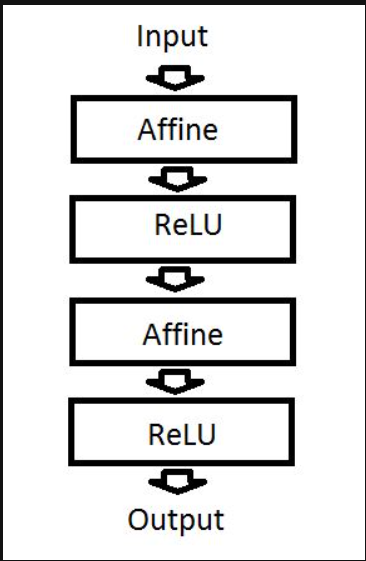
\includegraphics[width=0.5\textwidth,height=.5\textwidth]{nn_layer}
    \begin{choice} (2)
        * True
        *\correctchoice{False}
    \end{choice}
\end{exercise}
\begin{solution}
\end{solution}

\begin{exercise}
    Deep learning can be applied to which of the following NLP tasks?
    \begin{choice} (4)
        * Machine translation
        * Sentiment analysis
        * Question Answering system
        *\correctchoice{All of the above}
    \end{choice}
\end{exercise}
\begin{solution}
\end{solution}

\begin{exercise}
    Scenario 1: You are given data of the map of Arcadia city, with aerial photographs of the city and its outskirts. The task is to segment the areas into industrial land, farmland, and natural landmarks like rivers, mountains, etc. \\

    Scenario 2: You are given data of the map of Arcadia city, with detailed roads and distances between landmarks. This is represented as a graph structure. The task is to find out the nearest distance between two landmarks.\\

    Can deep learning be applied to Scenario 1 but not Scenario 2?
    \begin{choice} (2)
        * TRUE
        *\correctchoice{FALSE}
    \end{choice}
\end{exercise}
\begin{solution}
\end{solution}

\begin{exercise}
    Which of the following is a data augmentation technique used in image recognition tasks?
    \begin{choice} (7)
        * Horizontal flipping
        * Random cropping
        * Random scaling
        * Color jittering
        * Random translation
        * Random shearing
        *\correctchoice{All of these}
    \end{choice}
\end{exercise}
\begin{solution}
\end{solution}

\begin{exercise}
    Given an n-character word, we want to predict which character would be the n+1th character in the sequence. For example, our input is “predictio” (which is a 9-character word) and we have to predict what would be the 10th character.\\

    Which neural network architecture would be suitable to complete this task?
    \begin{choice} (4)
        * Fully-Connected Neural Network
        * Convolutional Neural Network
        *\correctchoice{Recurrent Neural Network}
        * Restricted Boltzmann Machine
    \end{choice}
\end{exercise}
\begin{solution}
\end{solution}

\begin{exercise}
    What is generally the sequence followed when building a neural network architecture for semantic segmentation for an image?
    \begin{choice} (2)
        *\correctchoice{Convolutional network on input and deconvolutional network on output}
        * Deconvolutional network on input and convolutional network on output
    \end{choice}
\end{exercise}
\begin{solution}
\end{solution}

\begin{exercise}
    A ReLU unit in neural network never gets saturated.
    \begin{choice} (2)
        *True
        *\correctchoice{False}
    \end{choice}
\end{exercise}
\begin{solution}
\end{solution}

\begin{exercise}
    What is the relationship between dropout rate and regularization?
    \begin{choice} (2)
        * Higher the dropout rate, higher is the regularization
        *\correctchoice{Higher the dropout rate, lower is the regularization}
    \end{choice}
\end{exercise}
\begin{solution}
\end{solution}

\begin{exercise}
    What is the technical difference between vanilla backpropagation algorithm and backpropagation through time (BPTT) algorithm?
    \begin{choice} (2)
        *\correctchoice{Unlike backprop, in BPTT we sum up gradients for corresponding weight for each time step}
        * Unlike backprop, in BPTT we subtract gradients for corresponding weight for each time step
    \end{choice}
\end{exercise}
\begin{solution}
\end{solution}

\begin{exercise}
    Exploding gradient problem is an issue in training deep networks where the gradient gets so large that the loss goes to an infinitely high value and then explodes.\\ What is the probable approach when dealing with the "Exploding Gradient" problem in RNNs?
    \begin{choice} (2)
        * Use modified architectures like LSTM and GRUs
        *\correctchoice{Gradient clipping}
        * Dropout
        * None of these
    \end{choice}
\end{exercise}
\begin{solution}
\end{solution}

\begin{exercise}
    There are many types of gradient descent algorithms. Two of the most notable ones are l-BFGS and SGD. l-BFGS is a second-order gradient descent technique whereas SGD is a first-order gradient descent technique.\\ In which of the following scenarios would you prefer l-BFGS over SGD?
    \begin{choice} (4)
        * Data is sparse
        * Number of parameters of neural network are small
        * \correctchoice{Both of them}
        * None of these
    \end{choice}
\end{exercise}
\begin{solution}
\end{solution}

\begin{exercise}
    Which of the following is not a direct prediction technique for NLP tasks?
    \begin{choice} (2)
        * Recurrent Neural Network
        * Skip-gram model
        *\correctchoice{PCA}
        * Convolutional Neural Network
    \end{choice}
\end{exercise}
\begin{solution}
\end{solution}

\begin{exercise}
    Which of the following would be the best for a non-continuous objective during optimization in deep neural net?
    \begin{choice} (4)
        * L-BFGS
        * SGD
        * AdaGrad
        *\correctchoice{Subgradient method}
    \end{choice}
\end{exercise}
\begin{solution}
\end{solution}

\begin{exercise}
    Which of the following is correct?
    \begin{choice} (4)
        * Dropout randomly masks the input weights to a neuron
        * Dropconnect randomly masks both input and output weights to a neuron
        *\correctchoice{1 is False and 2 is True}
        * Both 1 and 2 are True
    \end{choice}
\end{exercise}
\begin{solution}
    In dropout, neurons are dropped, whereas in dropconnect, connections are dropped. So, both input and output weights will be rendered useless in dropconnect, while only one of them should be dropped in dropconnect.
\end{solution}

\begin{exercise}
    While training a neural network for image recognition task, we plot the graph of training error and validation error for debugging.
    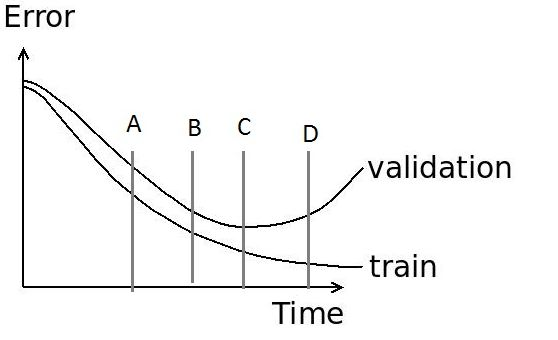
\includegraphics[width=.5\textwidth, height=.5\textwidth]{DL4}
    \begin{choice} (4)
        * A
        * B
        *\correctchoice{C}
        * D
    \end{choice}
\end{exercise}
\begin{solution}
    In dropout, neurons are dropped, whereas in dropconnect, connections are dropped. So, both input and output weights will be rendered useless in dropconnect, while only one of them should be dropped in dropconnect.
\end{solution}

\begin{exercise}
    Backpropagation works by first calculating the gradient of \_\_\_ and then propagating it backward.
    \begin{choice} (4)
        * Sum of squared error with respect to inputs
        * Sum of squared error with respect to weights
        *\correctchoice{Sum of squared error with respect to outputs}
        * None of the above
    \end{choice}
\end{exercise}
\begin{solution}
\end{solution}

\begin{exercise}
    Mini-Batch sizes when defining a neural network are preferred to be multiples of 2's such as 256 or 512. What is the reason behind it?
    \begin{choice} (4)
        * Gradient descent optimizes best when you use an even number
        *\correctchoice{Parallelization of the neural network is best when the memory is used optimally}
        * Losses are erratic when you don't use an even number
        * None of these
    \end{choice}
\end{exercise}
\begin{solution}
\end{solution}

\begin{exercise}
    As the length of a sentence increases, it becomes harder for a neural translation machine to perform as sentence meaning is represented by a fixed dimensional vector. To solve this, which of the following could we do?
    \begin{choice} (4)
        * Use recursive units instead of recurrent
        *\correctchoice{Use attention mechanism}
        * Use character-level translation
        * None of these
    \end{choice}
\end{exercise}
\begin{solution}
\end{solution}

\begin{exercise}
    A recurrent neural network can be unfolded into a fully connected neural network with infinite length.
    \begin{choice} (2)
        *\correctchoice{TRUE}
        * FALSE
    \end{choice}
\end{exercise}
\begin{solution}
\end{solution}

\begin{exercise}
    Which of the following is a bottleneck for deep learning algorithms?
    \begin{choice} (4)
        * Data related to the problem
        * CPU to GPU communication
        * GPU memory
        *\correctchoice{All of the above}
    \end{choice}
\end{exercise}
\begin{solution}
\end{solution}

\begin{exercise}
    When deriving a memory cell in memory networks, we choose to read values as vector values instead of scalars. Which type of addressing would this entail?
    \begin{choice} (2)
        *\correctchoice{Content-based addressing}
        * Location-based addressing
    \end{choice}
\end{exercise}
\begin{solution}
\end{solution}

\begin{exercise}
    It is generally recommended to replace pooling layers in the generator part of convolutional generative adversarial nets with \_\_\_\_\_\_\_\_\_\_?
    \begin{choice} (4)
        * Affine layer
        * Strided convolutional layer
        *\correctchoice{Fractional strided convolutional layer}
        * ReLU layer
    \end{choice}
\end{exercise}
\begin{solution}
\end{solution}

\begin{exercise}
    Which of the following statements is true with respect to GRU?
    \begin{choice} (4)
        *Units with short-term dependencies have a very active reset gate.
        *Units with long-term dependencies have a very active update gate.
        * None of them
        * \correctchoice{Both 1 and 2}
    \end{choice}
\end{exercise}
\begin{solution}
\end{solution}

\begin{exercise}
    If the calculation of the reset gate in a GRU unit is close to 0, which of the following would occur?
    \begin{choice} (2)
        *\correctchoice{Previous hidden state would be ignored}
        * Previous hidden state would not be ignored
    \end{choice}
\end{exercise}
\begin{solution}
\end{solution}

\begin{exercise}
    If the calculation of the update gate in a GRU unit is close to 1, which of the following would occur?
    \begin{choice} (2)
        * Forgets the information for future time steps
        *\correctchoice{Copies the information through many time steps}
    \end{choice}
\end{exercise}
\begin{solution}
\end{solution}

\begin{exercise}
    Dropout technique is not an advantageous technique for which of the following layers?
    \begin{choice} (4)
        * Affine layer
        * Convolutional layer
        *\correctchoice{RNN layer}
        * None of these
    \end{choice}
\end{exercise}
\begin{solution}
\end{solution}

\begin{exercise}
    Suppose your task is to predict the next few notes of a song when you are given the preceding segment of the song. Which architecture of a neural network would be better suited to solve the problem?
    \begin{choice} (4)
        * End-to-End fully connected neural network
        * \correctchoice{CNN followed by recurrent units}
        * Neural Turing Machine
        * None of these
    \end{choice}
\end{exercise}
\begin{solution}
\end{solution}

% https://aimcqs.com/convolutional-neural-networks
\begin{exercise}
    What is the primary purpose of a Convolutional Neural Network (CNN)?
    \begin{choice} (4)
        * Object detection
        * \correctchoice{Image classification}
        * Text generation
        * Reinforcement learning
    \end{choice}
\end{exercise}
\begin{solution}
\end{solution}

\begin{exercise}
    Which layer type is typically used to extract local features in a CNN?
    \begin{choice} (4)
        * \correctchoice{Convolutional layer}
        * Pooling layer
        * Fully connected layer
        * Activation layer
    \end{choice}
\end{exercise}
\begin{solution}
\end{solution}

\begin{exercise}
    What is the advantage of using convolutional layers in a CNN?
    \begin{choice} (4)
        * \correctchoice{They can capture local spatial patterns in the input data}
        * They can handle sequential data
        * They can generate synthetic data
        * They can capture local spatial patterns in the input data
    \end{choice}
\end{exercise}
\begin{solution}
\end{solution}

\begin{exercise}
    What is the purpose of the pooling layer in a CNN?
    \begin{choice} (4)
        * To introduce non-linearity to the network
        * \correctchoice{To reduce the spatial dimensions of the feature maps}
        * To adjust the weights and biases of the network
        * To compute the gradients for backpropagation
    \end{choice}
\end{exercise}
\begin{solution}
\end{solution}

\begin{exercise}
    Which activation function is commonly used in the convolutional layers of a CNN?
    \begin{choice} (4)
        * Sigmoid
        * \correctchoice{ReLU (Rectified Linear Unit)}
        * Tanh (Hyperbolic Tangent)
        * Softmax
    \end{choice}
\end{exercise}
\begin{solution}
\end{solution}

\begin{exercise}
    What is the purpose of the stride parameter in a convolutional layer?
    \begin{choice} (4)
        * To determine the size of the receptive field
        * \correctchoice{To control the step size of the convolution operation}
        * To adjust the learning rate during training
        * None of the above
    \end{choice}
\end{exercise}
\begin{solution}
\end{solution}

\begin{exercise}
    Which layer type is used to reduce the spatial dimensions in a CNN?
    \begin{choice} (4)
        * Convolutional layer
        * \correctchoice{Pooling layer}
        * Fully connected layer
        * Activation layer
    \end{choice}
\end{exercise}
\begin{solution}
\end{solution}

\begin{exercise}
    What is the purpose of the padding parameter in a convolutional layer?
    \begin{choice} (4)
        * To adjust the learning rate during training
        * \correctchoice{To prevent the reduction of spatial dimensions}
        * To regularize the network and prevent overfitting
        * None of the above
    \end{choice}
\end{exercise}
\begin{solution}
\end{solution}

\begin{exercise}
    Which layer type is responsible for making final predictions in a CNN?
    \begin{choice} (4)
        * Convolutional layer
        * Pooling layer
        * \correctchoice{Fully connected layer}
        * Activation layer
    \end{choice}
\end{exercise}
\begin{solution}
\end{solution}

\begin{exercise}
    What is the purpose of the fully connected layers in a CNN?
    \begin{choice} (4)
        * \correctchoice{To capture global patterns and make predictions}
        * To reduce the spatial dimensions of the input data
        * To apply non-linear transformations to the feature maps
        * To initialize the weights and biases of the network
    \end{choice}
\end{exercise}
\begin{solution}
\end{solution}


\begin{exercise}
    Which layer type is responsible for applying non-linear transformations to the feature maps in a CNN?
    \begin{choice} (4)
        * Convolutional layer
        * Pooling layer
        * Fully connected layer
        * \correctchoice{Activation layer}
    \end{choice}
\end{exercise}
\begin{solution}
\end{solution}

\begin{exercise}
    What is the purpose of dropout regularization in a CNN?
    \begin{choice} (4)
        * \correctchoice{To randomly disable neurons during training to prevent overfitting}
        * To adjust the learning rate during training
        * To increase the number of layers in the network
        * None of the above
    \end{choice}
\end{exercise}
\begin{solution}
\end{solution}

\begin{exercise}
    Which layer type is responsible for backpropagating the gradients and updating the network's parameters in a CNN?
    \begin{choice} (4)
        * Convolutional layer
        * Pooling layer
        * \correctchoice{Fully connected layer}
        * Activation layer
    \end{choice}
\end{exercise}
\begin{solution}
\end{solution}

\begin{exercise}
    What is the primary advantage of using a CNN over a fully connected neural network for image processing tasks?
    \begin{choice} (4)
        * CNNs have a higher training speed
        * CNNs can handle sequential data
        * CNNs have a higher number of neurons
        * \correctchoice{CNNs can capture local spatial patterns in the input data}
    \end{choice}
\end{exercise}
\begin{solution}
\end{solution}

\begin{exercise}
    Which layer type is responsible for parameter sharing in a CNN?
    \begin{choice} (4)
        * \correctchoice{Convolutional layer}
        * Pooling layer
        * Fully connected layer
        * Activation layer
    \end{choice}
\end{exercise}
\begin{solution}
\end{solution}

\begin{exercise}
    What is the purpose of the receptive field in a convolutional layer?
    \begin{choice} (4)
        * To determine the number of filters in the layer
        * To determine the size of the feature maps
        * \correctchoice{To specify the size of the local region for the convolution operation}
        * None of the above
    \end{choice}
\end{exercise}
\begin{solution}
\end{solution}

\begin{exercise}
    Which layer type is responsible for spatial downsampling in a CNN?
    \begin{choice} (4)
        * Convolutional layer
        * \correctchoice{Pooling layer}
        * Fully connected layer
        * Activation layer
    \end{choice}
\end{exercise}
\begin{solution}
\end{solution}

\begin{exercise}
    What is the purpose of the filter/kernel in a convolutional layer?
    \begin{choice} (4)
        * To determine the number of neurons in the layer
        * To specify the size of the feature maps
        * \correctchoice{To extract local features from the input data}
        * None of the above
    \end{choice}
\end{exercise}
\begin{solution}
\end{solution}

\begin{exercise}
    Which layer type is commonly used in CNNs to normalize the input data?
    \begin{choice} (4)
        * Convolutional layer
        * Pooling layer
        * \correctchoice{Batch normalization layer}
        * Activation layer
    \end{choice}
\end{exercise}
\begin{solution}
\end{solution}

\begin{exercise}
    What is the primary goal of training a CNN?
    \begin{choice} (4)
        * \correctchoice{To minimize the prediction error on the training data}
        * To maximize the number of layers in the network
        * To achieve 100% accuracy on the test data
        * None of the above
    \end{choice}
\end{exercise}
\begin{solution}
\end{solution}

---

\begin{exercise}
    Which layer type is responsible for introducing translation invariance in a CNN?
    \begin{choice} (4)
        * \correctchoice{Convolutional layer}
        * Pooling layer
        * Fully connected layer
        * Activation layer
    \end{choice}
\end{exercise}
\begin{solution}
\end{solution}

\begin{exercise}
    What is the purpose of the output layer in a CNN?
    \begin{choice} (4)
        * \correctchoice{To compute the predicted output based on the final feature representation}
        * To reduce the spatial dimensions of the input data
        * To apply non-linear transformations to the feature maps
        * To initialize the weights and biases of the network
    \end{choice}
\end{exercise}
\begin{solution}
\end{solution}

\begin{exercise}
    What is the purpose of zero-padding in a CNN?
    \begin{choice} (4)
        * To adjust the learning rate during training
        * \correctchoice{To prevent the reduction of spatial dimensions}
        * To regularize the network and prevent overfitting
        * None of the above
    \end{choice}
\end{exercise}
\begin{solution}
\end{solution}

\begin{exercise}
    Which layer type is commonly used in CNNs for semantic segmentation tasks?
    \begin{choice} (4)
        * Convolutional layer
        * Pooling layer
        * Fully connected layer
        * \correctchoice{Upsampling layer}
    \end{choice}
\end{exercise}
\begin{solution}
\end{solution}

\begin{exercise}
    What is the purpose of the loss function in CNN training?
    \begin{choice} (4)
        * \correctchoice{To measure the prediction error and guide the learning process}
        * To initialize the weights and biases of the network
        * To adjust the learning rate during training
        * None of the above
    \end{choice}
\end{exercise}
\begin{solution}
\end{solution}

\begin{exercise}
    Which layer type is commonly used in CNNs to introduce non-linearity?
    \begin{choice} (4)
        * Convolutional layer
        * Pooling layer
        * Fully connected layer
        * \correctchoice{Activation layer}
    \end{choice}
\end{exercise}
\begin{solution}
\end{solution}

\begin{exercise}
    What is the purpose of the learning rate in CNN training?
    \begin{choice} (4)
        * \correctchoice{To control the step size of the parameter updates during optimization}
        * To adjust the size of the filters in the convolutional layers
        * To increase the number of layers in the network
        * None of the above
    \end{choice}
\end{exercise}
\begin{solution}
\end{solution}

\begin{exercise}
    Which layer type is responsible for feature extraction in a CNN?
    \begin{choice} (4)
        * \correctchoice{Convolutional layer}
        * Pooling layer
        * Fully connected layer
        * Activation layer
    \end{choice}
\end{exercise}
\begin{solution}
\end{solution}

\begin{exercise}
    What is the purpose of data augmentation in CNN training?
    \begin{choice} (4)
        * To increase the number of layers in the network
        * \correctchoice{To introduce noise and variations in the training data}
        * To adjust the learning rate during training
        * None of the above
    \end{choice}
\end{exercise}
\begin{solution}
\end{solution}

\begin{exercise}
    Which layer type is commonly used in CNNs to handle variable-sized inputs?
    \begin{choice} (4)
        * Convolutional layer
        * Pooling layer
        * Fully connected layer
        * \correctchoice{None of the above}
    \end{choice}
\end{exercise}
\begin{solution}
\end{solution}


---

\begin{exercise}
    What is the primary purpose of a Recurrent Neural Network (RNN)?
    \begin{choice} (4)
        * Image classification
        * \correctchoice{Text generation}
        * Reinforcement learning
        * Object detection
    \end{choice}
\end{exercise}
\begin{solution}
\end{solution}

\begin{exercise}
    Which layer type is typically used to capture sequential dependencies in an RNN?
    \begin{choice} (4)
        * Input layer
        * \correctchoice{Hidden layer}
        * Output layer
        * Activation layer
    \end{choice}
\end{exercise}
\begin{solution}
\end{solution}

\begin{exercise}
    What is the advantage of using recurrent layers in an RNN?
    \begin{choice} (4)
        * They can handle non-linear transformations
        * They can handle variable-length inputs
        * They can generate synthetic data
        * \correctchoice{They can capture temporal dependencies in the input data}
    \end{choice}
\end{exercise}
\begin{solution}
\end{solution}

\begin{exercise}
    What is the purpose of the hidden state in an RNN?
    \begin{choice} (4)
        * \correctchoice{To store the information from the previous time step}
        * To adjust the learning rate during training
        * To compute the gradients for backpropagation
        * None of the above
    \end{choice}
\end{exercise}
\begin{solution}
\end{solution}

\begin{exercise}
    Which activation function is commonly used in the recurrent layers of an RNN?
    \begin{choice} (4)
        * ReLU (Rectified Linear Unit)
        * Sigmoid
        * \correctchoice{Tanh (Hyperbolic Tangent)}
        * Softmax
    \end{choice}
\end{exercise}
\begin{solution}
\end{solution}

\begin{exercise}
    What is the purpose of the time step parameter in an RNN?
    \begin{choice} (4)
        * To determine the number of recurrent layers in the network
        * To adjust the learning rate during training
        * \correctchoice{To specify the length of the input sequence}
        * None of the above
    \end{choice}
\end{exercise}
\begin{solution}
\end{solution}

\begin{exercise}
    Which layer type is commonly used to initialize the hidden state in an RNN?
    \begin{choice} (4)
        * Input layer
        * \correctchoice{Hidden layer}
        * Output layer
        * Activation layer
    \end{choice}
\end{exercise}
\begin{solution}
\end{solution}

\begin{exercise}
    What is the purpose of the bidirectional RNN architecture?
    \begin{choice} (4)
        * \correctchoice{To handle sequential data in both forward and backward directions}
        * To reduce the computational complexity of the network
        * To adjust the learning rate during training
        * None of the above
    \end{choice}
\end{exercise}
\begin{solution}
\end{solution}

\begin{exercise}
    Which layer type is responsible for making final predictions in an RNN?
    \begin{choice} (4)
        * Input layer
        * Hidden layer
        * \correctchoice{Output layer}
        * Activation layer
    \end{choice}
\end{exercise}
\begin{solution}
\end{solution}

\begin{exercise}
    What is the purpose of the recurrent connection in an RNN?
    \begin{choice} (4)
        * \correctchoice{To propagate the hidden state across different time steps}
        * To adjust the weights and biases of the network
        * To reduce the dimensionality of the input data
        * None of the above
    \end{choice}
\end{exercise}
\begin{solution}
\end{solution}

\begin{exercise}
    Which layer type is commonly used in RNNs for sequence-to-sequence tasks?
    \begin{choice} (4)
        * Input layer
        * Hidden layer
        * Output layer
        * \correctchoice{Attention layer}
    \end{choice}
\end{exercise}
\begin{solution}
\end{solution}

\begin{exercise}
    What is the purpose of the backpropagation through time (BPTT) algorithm in RNN training?
    \begin{choice} (4)
        * \correctchoice{To compute the gradients and update the network's parameters}
        * To adjust the learning rate during training
        * To prevent overfitting by regularizing the model
        * None of the above
    \end{choice}
\end{exercise}
\begin{solution}
\end{solution}

\begin{exercise}
    Which layer type is commonly used in RNNs to handle variable-length inputs?
    \begin{choice} (4)
        * \correctchoice{Input layer}
        * Hidden layer
        * Output layer
        * None of the above
    \end{choice}
\end{exercise}
\begin{solution}
\end{solution}

\begin{exercise}
    What is the purpose of the initial hidden state in an RNN?
    \begin{choice} (4)
        * \correctchoice{To provide the starting point for the recurrent computation}
        * To adjust the learning rate during training
        * To compute the gradients for backpropagation
        * None of the above
    \end{choice}
\end{exercise}
\begin{solution}
\end{solution}

\begin{exercise}
    Which layer type is responsible for handling the output at each time step in an RNN?
    \begin{choice} (4)
        * Input layer
        * Hidden layer
        * \correctchoice{Output layer}
        * Activation layer
    \end{choice}
\end{exercise}
\begin{solution}
\end{solution}

\begin{exercise}
    What is the purpose of the teacher forcing technique in RNN training?
    \begin{choice} (4)
        * To adjust the learning rate during training
        * \correctchoice{To propagate the gradients through time}
        * To reduce the computational complexity of the network
        * None of the above
    \end{choice}
\end{exercise}
\begin{solution}
\end{solution}

\begin{exercise}
    Which layer type is commonly used in RNNs for language modeling tasks?
    \begin{choice} (4)
        * Input layer
        * Hidden layer
        * \correctchoice{Output layer}
        * None of the above
    \end{choice}
\end{exercise}
\begin{solution}
\end{solution}

\begin{exercise}
    What is the purpose of the sequence-to-vector architecture in an RNN?
    \begin{choice} (4)
        * \correctchoice{To process an input sequence and produce a fixed-length representation}
        * To adjust the weights and biases of the network
        * To reduce the dimensionality of the input data
        * None of the above
    \end{choice}
\end{exercise}
\begin{solution}
\end{solution}

\begin{exercise}
    Which layer type is responsible for introducing non-linearity in an RNN?
    \begin{choice} (4)
        * Input layer
        * Hidden layer
        * Output layer
        * \correctchoice{Activation layer}
    \end{choice}
\end{exercise}
\begin{solution}
\end{solution}

\begin{exercise}
    What is the purpose of the forget gate in a Gated Recurrent Unit (GRU)?
    \begin{choice} (4)
        * \correctchoice{To control the flow of information from the previous hidden state}
        * To adjust the learning rate during training
        * To compute the gradients for backpropagation
        * None of the above
    \end{choice}
\end{exercise}
\begin{solution}
\end{solution}

\begin{exercise}
    Which layer type is commonly used in RNNs for machine translation tasks?
    \begin{choice} (4)
        * Input layer
        * Hidden layer
        * Output layer
        * \correctchoice{Attention layer}
    \end{choice}
\end{exercise}
\begin{solution}
\end{solution}

\begin{exercise}
    What is the purpose of the peephole connections in a Long Short-Term Memory (LSTM) network?
    \begin{choice} (4)
        * \correctchoice{To allow the cell state to influence the gating mechanisms}
        * To adjust the learning rate during training
        * To introduce non-linearity to the network
        * None of the above
    \end{choice}
\end{exercise}
\begin{solution}
\end{solution}

\begin{exercise}
    Which layer type is responsible for handling variable-length outputs in an RNN?
    \begin{choice} (4)
        * Input layer
        * Hidden layer
        * \correctchoice{Output layer}
        * None of the above
    \end{choice}
\end{exercise}
\begin{solution}
\end{solution}

\begin{exercise}
    What is the purpose of the cell state in an LSTM network?
    \begin{choice} (4)
        * \correctchoice{To store long-term dependencies in the input sequence}
        * To adjust the learning rate during training
        * To compute the gradients for backpropagation
        * None of the above
    \end{choice}
\end{exercise}
\begin{solution}
\end{solution}

\begin{exercise}
    Which layer type is commonly used in RNNs for speech recognition tasks?
    \begin{choice} (4)
        * Input layer
        * Hidden layer
        * \correctchoice{Output layer}
        * None of the above
    \end{choice}
\end{exercise}
\begin{solution}
\end{solution}

\begin{exercise}
    What is the purpose of the input gate in an LSTM network?
    \begin{choice} (4)
        * \correctchoice{To control the flow of information from the current input}
        * To adjust the learning rate during training
        * To introduce non-linearity to the network
        * None of the above
    \end{choice}
\end{exercise}
\begin{solution}
\end{solution}

\begin{exercise}
    Which layer type is responsible for handling variable-length inputs and outputs in an RNN?
    \begin{choice} (4)
        * Input layer
        * Hidden layer
        * Output layer
        * \correctchoice{None of the above}
    \end{choice}
\end{exercise}
\begin{solution}
\end{solution}

\begin{exercise}
    What is the purpose of the output gate in an LSTM network?
    \begin{choice} (4)
        * \correctchoice{To control the flow of information to the current output}
        * To adjust the learning rate during training
        * To introduce non-linearity to the network
        * None of the above
    \end{choice}
\end{exercise}
\begin{solution}
\end{solution}

\begin{exercise}
    Which layer type is commonly used in RNNs for time series prediction tasks?
    \begin{choice} (4)
        * Input layer
        * Hidden layer
        * \correctchoice{Output layer}
        * None of the above
    \end{choice}
\end{exercise}
\begin{solution}
\end{solution}

\begin{exercise}
    What is the purpose of the reset gate in a Gated Recurrent Unit (GRU)?
    \begin{choice} (4)
        * \correctchoice{To reset the hidden state based on the current input}
        * To adjust the learning rate during training
        * To introduce non-linearity to the network
        * None of the above
    \end{choice}
\end{exercise}
\begin{solution}
\end{solution}


\newpage
\begin{multicols*}{2}
    \printsolutions*
\end{multicols*}
\end{document}